\documentclass[11pt]{article}
\usepackage{graphicx}
\usepackage{hyperref}
%\usepackage{appendix}
\usepackage{amsmath}
\usepackage{amssymb}
\usepackage{float}
\usepackage{commath}
%\usepackage{siunitx}
%\sisetup{detect-all}
\usepackage[a4paper,margin=20mm]{geometry}
\numberwithin{equation}{section}
\setlength{\parskip}{\baselineskip}
\setlength{\parindent}{0pt}
\hypersetup{
    colorlinks=true,
    linkcolor=magenta,
    filecolor=magenta,      
    urlcolor=magenta,
}
\urlstyle{same}
\begin{document}
\title{\textbf{UCL Mechanical Engineering 2020/2021}\\ENGF0004 Coursework 1}
\author{NCWT3}
\maketitle
\section{Question One}
\subsection*{a}
\subsection*{b}
We are given:
\begin{align}
	f(x) &= \frac{x}{\sqrt{1-x}}\\
	f(x) &= x\left( 1 - x \right)^{-\frac{1}{2}}
\end{align}
Differentiating three times yields:
\begin{align}
	f'(x) &= \left(1 - x \right)^{-\frac{1}{2}} + \frac{x}{2} \left( 1-x\right)^{-\frac{3}{2}}\\
	f''(x) &= \frac{1}{2} \left( 1- x\right)^{-\frac{3}{2}} + \frac{1}{2} \left( 1- x\right)^{-\frac{3}{2}} + \frac{3x}{4} \left( 1-x \right)^{-\frac{5}{2}}\\
	&= \left( 1-x \right)^{-\frac{3}{2}} + \frac{3x}{4} \left( 1-x \right)^{-\frac{5}{2}} \\
	f'''(x) &= \frac{3}{2} \left( 1-x \right)^{-\frac{5}{2}} + \frac{3}{4} \left( 1-x \right)^{-\frac{5}{2}} + \frac{15x}{8} \left( 1-x \right)^{-\frac{7}{2}}\\
	&= \frac{9}{4} \left( 1-x \right)^{-\frac{5}{2}} + \frac{15x}{8} \left( 1-x \right)^{-\frac{7}{2}}
\end{align}
Inputting $x=0$:
\begin{align}
	f(0) &= 0 \cdot \left( 1 - 0 \right)^{-\frac{1}{2}}\\
	&= 0\\
	f'(0) &= \left(1 - 0 \right)^{-\frac{1}{2}} + \frac{0}{2} \left( 1-0\right)^{-\frac{3}{2}}\\
	&= 1\\
	f''(0) &= \left( 1-0 \right)^{-\frac{3}{2}} + \frac{3\cdot 0}{4} \left( 1-0 \right)^{-\frac{5}{2}}\\
	&= 1\\
	f'''(0) &= \frac{9}{4} \left( 1-0 \right)^{-\frac{5}{2}} + \frac{15 \cdot 0}{8} \left( 1-0 \right)^{-\frac{7}{2}}\\
	&= \frac{9}{4}
\end{align}
General form of Maclaurin series:
\begin{align}
	f(x) \approx f(0) + \frac{x}{1!}f'(0) + \frac{x^2}{2!}f''(0) + \frac{x^3}{3!}f'''(0) + ... \label{macser}
\end{align}
Inputting the above variables into Eq.\ref{macser}:
\begin{align}
	f(x) \approx x + \frac{x^2}{2} + \frac{3x^3}{8}	
\end{align}
\subsection*{c}
\subsubsection*{i}
We are given:
\begin{align}
E = \frac{kq}{x^2}
\end{align}
Sum of electric fields due to both charged particles is:
\begin{align}
	E &= \frac{ke}{\left( x-r \right)^2} - \frac{ke}{\left( x+r \right)^2}\\
	&= ke \left[ \frac{1}{x^2\left( 1 - \frac{r}{x} \right)^2} - \frac{1}{x^2\left( 1 + \frac{r}{x} \right)^2} \right]\\
	E&= \frac{ke}{x^2} \left[ \left( 1- y \right)^{-2} - \left( 1 + y\right)^{-2} \right]
\end{align}
Where $y =\frac{r}{x}$.
\subsubsection*{ii}
Calculation of constants to be used in Maclaurin series expansion:
\begin{equation*}
	\begin{aligned}[c]
		f(y) &= \left( 1 - y \right)^{-2}\\
		f'(y) &= 2\left(1-y\right)^{-3}\\
		f''(y) &= 6\left(1-y\right)^{-4}\\
		f'''(y) &= 24\left(1-y\right)^{-5}
	\end{aligned}
	\makebox[2cm]{}
	\begin{aligned}[c]
		f(0) &= 1\\
		f'(0) &= 2\\
		f''(0) &= 6\\
		f'''(0) &= 24\\
	\end{aligned}
\end{equation*}
\begin{equation*}
	\begin{aligned}[c]
		g(y) &= \left( 1 + y \right)^{-2}\\
		g'(y) &= -2\left(1+y\right)^{-3}\\
		g''(y) &= 6\left(1+y\right)^{-4}\\
		g'''(y) &= -24\left(1+y\right)^{-5}
	\end{aligned}
	\makebox[2cm]{}
	\begin{aligned}[c]
		g(0) &= 1\\
		g'(0) &= -2\\
		g''(0) &= 6\\
		g'''(0) &= -24\\
	\end{aligned}
\end{equation*}
Inputting the above variables into Eq.\ref{macser}:
\begin{align}
	f(y) &\approx 1 + \frac{2 y}{1!} + \frac{6y^2}{2!} + \frac{24y^3}{3!} + ...\\
	f(y) &\approx 1 + 2y + 3y^2 + 4y^3 \\ 
	g(y) &\approx 1 - \frac{2 y}{1!} + \frac{6y^2}{2!} - \frac{24y^3}{3!} + ...\\
	g(y) &\approx 1 - 2y + 3y^2 - 4y^2
\end{align}
Substitution:
\begin{align}
	E &\approx \frac{ke}{x^2} \left[ f(y) - g(y)\right]\\
	&\approx \frac{ke}{x^2} \left[ 1 + 2y + 3y^2 + 4y^3 - 1 + 2y - 3y^2 + 4y^3 \right]\\
	&\approx \frac{ke}{x^2}\left[ 4y + 8y^3 \right]\\
	E &\approx \frac{4ke}{x^2}\left[ y + 2y^3 \right]
\end{align}
\subsubsection*{iii}
$y = 0.01$. Exact:
\begin{align}
	E_E &= \frac{ke}{x^2} \left[\left(1-0.01\right)^{-2}-\left(1+0.01\right)^{-2}\right]\\
	E_E &= \frac{ke}{x^2} \left[0.0400080012\right]\\
\end{align}
Approximation:
\begin{align}
	E_A &= \frac{ke}{x^2} \left[0.01 + 2\left(0.01\right)^3\right]\\
	E_A &= \frac{ke}{x^2} \left[0.010002\right]
\end{align}
Percentage error:
\begin{align}
	\frac{E_A}{E_E} \cdot 100 = \frac{0.010002}{0.0400080012} \cdot 100 = 25\% \textrm{ error (2sf)}
\end{align}
\subsection*{d}
We are given:
\begin{align}
	y'' - 2y' + y = te^t\\
	y(0) = 0, \ y'(0)=1
\end{align}
Laplace transformation (from tables):
\begin{gather}
	\mathcal{L} \{ y''\} - 2\mathcal{L} \{ y'\} + \mathcal{L} \{ y\} = \mathcal{L} \{te^t \}\\
	s^2 Y(s) - sy(0) - y'(0) - 2\left(sY(s) - y(0)\right) + Y(s) = \frac{1!}{\left(s-1\right)^2}\\
	s^2 Y(s) -1 -2(sY(s) - 1) + Y(s) = \frac{1}{\left(s-1\right)^2}\\
	Y(s)\left[s^2-2s+1\right] = \frac{1}{\left(s-1\right)^2}\\
	Y(s) = \frac{1}{\left(s-1\right)^2\left(s^2-2s+1\right)}\\
	= \frac{1}{\left(s-1\right)^2\left(s-1\right)^2}\\
	Y(s) = \frac{1}{\left(s-1\right)^4} 
\end{gather}
\subsection*{e}
\subsubsection*{i}
$a =1 \therefore -3 \leq t \leq 3$. Sketch:
\begin{figure}[H]
	\centering
	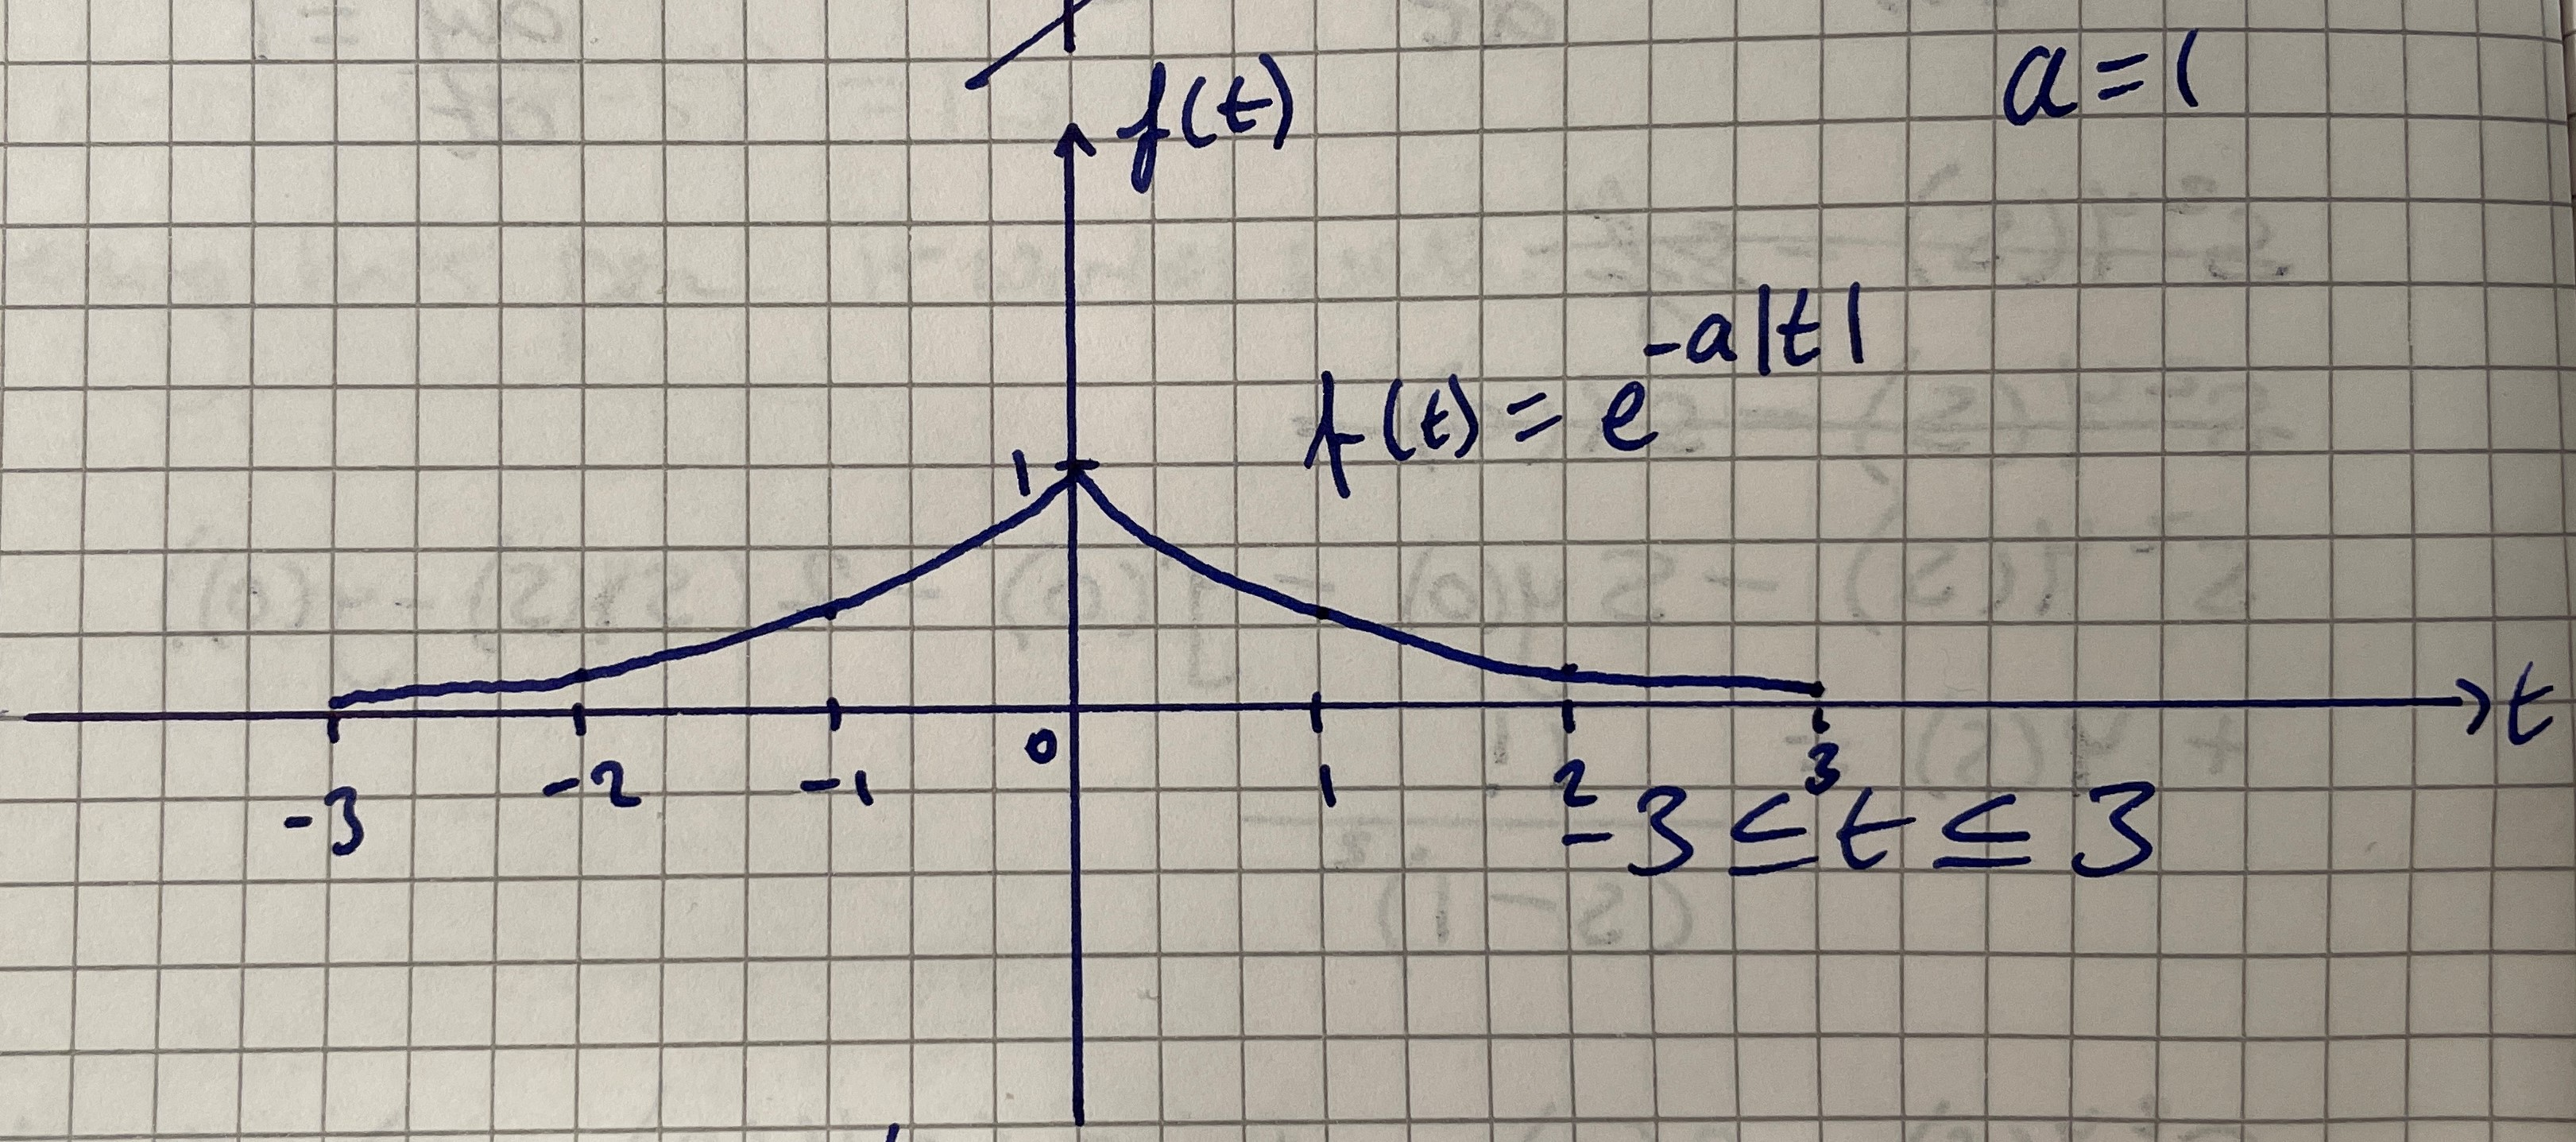
\includegraphics[width = 0.7\textwidth]{./img/q1ei.JPG}
	\caption{}
\end{figure}
\subsubsection*{ii}
\begin{align}
	F(u) &= \int_{t=-\infty}^{0}e^{at}e^{-j2\pi u t}  \,\dif t + \int_{t=0}^{\infty} e^{-at} e^{-j2\pi u t}\,\dif t\\
	&= \int_{t=-\infty}^{0}e^{t(a - j2\pi u)}  \,\dif t + \int_{t=0}^{\infty} e^{-t(a + j2\pi u)}\,\dif t\\
	&= \left. \frac{1}{\left(a - j2\pi u\right)}e^{-t\left(a - j2\pi u\right)} \right|_{t = -\infty}^0 + \left. \frac{1}{-\left(a + j2\pi u\right)}e^{-t\left(a + j2\pi u\right)} \right|_{t=0}^\infty\\
	&= \frac{1}{a - j2\pi u} + \frac{1}{a + j2\pi u}\\
	&= \frac{a + j2\pi u + a - j2\pi u}{a^2 + 4\pi^2 u^2}\\
	F(u) &= \frac{2a}{a^2 + 4\pi^2u^2}
\end{align}
\subsubsection*{iii}
Substituting $\omega = 2\pi u$, $\omega^2 = 4\pi^2 u^2$:
\begin{align}
	F(\omega) = \frac{2a}{a^2 + \omega^2}
\end{align}
\begin{figure}[H]
	\centering
	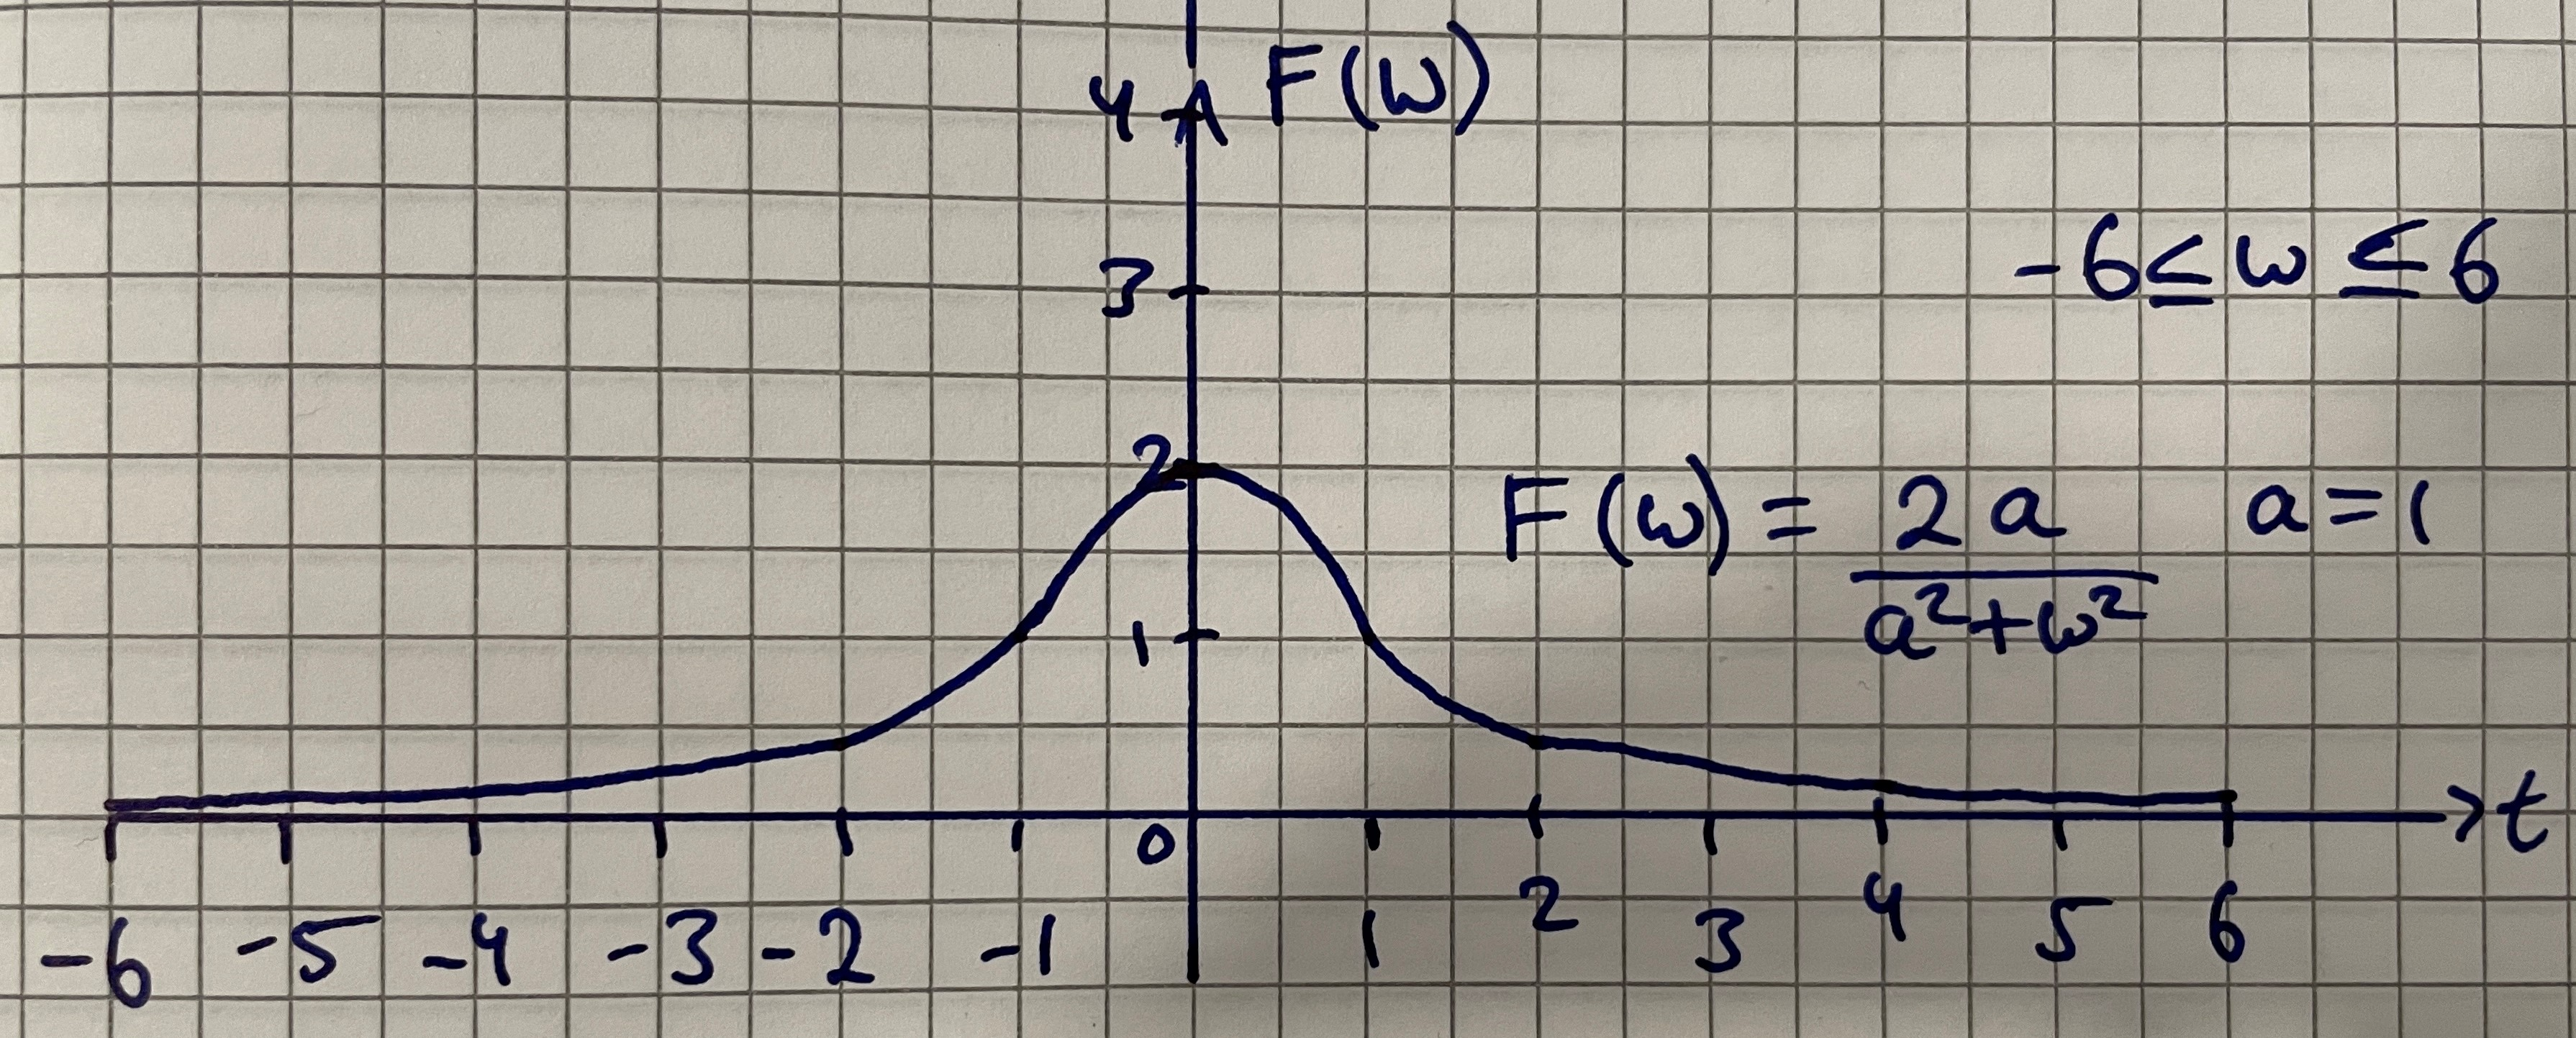
\includegraphics[width = 0.7\textwidth]{./img/q1eiii.JPG}
	\caption{}
\end{figure}
\subsubsection*{iv}
\subsubsection*{v}
\section{Question Two}
\subsection*{a}
\subsubsection*{i}
\begin{align}
	\frac{\partial u}{\partial t} = k \frac{\partial^2 u}{\partial x^2}
\end{align}
We know that $u(x,t) = X(x)T(t)$. Substituting:
\begin{align}
	\frac{\partial XT}{\partial t} &= k\frac{\partial^2 XT}{\partial x^2}\\
	X\frac{\partial T}{\partial t} &= kT\frac{\partial^2 X}{\partial x^2}
\end{align}
Divide by $XTk$:
\begin{align}
	\frac{1}{kT}\frac{\partial T}{\partial t} = \frac{1}{X}\frac{\partial^2 X}{\partial x^2} &= -\mu\\
	\frac{\partial T}{\partial t} + k\mu T &= 0\\
	T'(t) &= -\mu k T(t)\\
	\frac{\partial^2 X}{\partial x^2} + \mu X &= 0\\
	-X''(x) &= \mu X(x)
\end{align}
\subsubsection*{ii}
\begin{align}
	X''(x) + \mu X(x) &= 0\\
	\textrm{Let } X(x) &= e^{mx}\\
	X'(x) &= me^{mx}\\
	X''(x) &= m^2e^{mx}\\
	m^2 + \mu &= 0\\
	m &= \pm j\sqrt{\mu}\\
\end{align}
General solution:
\begin{align}
	X(x) = A\cos\left(\sqrt{\mu}x\right) + B\sin\left(\sqrt{\mu}x\right)
\end{align}
Boundary conditions:
\begin{align}
	u\left(0,t\right) &= 0\\
	X(0)T(t) &= 0\\
\end{align}
We require that $X(0) = 0$. Hence:
\begin{align}
	X(0) &= A\cos\left(0\right) + B\sin\left(0\right)\\
	\therefore A &= 0\\
	X(x) &= B \sin\left(\sqrt{\mu}x\right)\\
	u\left(l,t\right) &= 0\\
	X(l) &= B\sin\left(\sqrt{\mu}x\right) = 0\\
	\sqrt{\mu}x &= n\pi \textrm{ where } n = 1, \ 2, \ 3, \ ... \\
	\mu &= \frac{n^2 \pi^2}{x^2}
\end{align}
\subsubsection*{iii}
\subsection*{b}
\subsubsection*{i}
\subsubsection*{ii}
\subsubsection*{iii}
\subsubsection*{iv}
\subsubsection*{v}
\end{document}